\documentclass{beamer}
%\usepackage{beamerthemeshadow}
\usetheme{Warsaw}
\usepackage{latexsym,amsbsy,amsopn,amstext,xcolor,multicol,amsmath}
\usepackage{amssymb,graphicx,wrapfig,fancybox}
\usepackage{pgf,pgfarrows,pgfnodes,pgfautomata,pgfheaps,pgfshade}
\usepackage{booktabs}
\usepackage{subfloat}
\usepackage{}
\usecolortheme{}
\graphicspath{{figures/}}

\begin{document}

\title{Group Report}
\subtitle{Measure of the branching fraction of\\ decay $J/\psi \rightarrow \Omega {\pi}^+ \pi^+ \pi^- \pi^-$}
\author{Ma Hsuning}
\institute{physics of NKU}
\date{\today}
\frame{\titlepage}

\section{Introduction}
\subsection{}
\begin{frame}{Introduction}
\begin{itemized}
\item The process we are researching is the decay below
\begin{center}
$J/\psi &\rightarrow& \Omega\, {\pi}^+ \pi^+ \pi^- \pi^-$\\
$\Omega &\rightarrow&\pi^0\pi^-\pi^+$\\
$\pi^0 &\rightarrow& 2\gamma$\\
\end{center}

\item The Measure of branching fraction is accomplished via the formula below\\
		\bigskip
$$N^{tot}_{data}\times Br(J\!/\!\psi\!\rightarrow\!\Omega\;4\pi)\times Br(\Omega\!\rightarrow\!3\pi)\times Br(\pi^0\!\rightarrow\!2\gamma)\times \epsilon=N^{obs}_{data} \eqno{(*)}$$
\end{itemized}
\end{frame}

\section{Measure of the branching fraction}
\subsection{}

\begin{frame}{Measure of $N^{obs}_{data}$}
After running the data samples, we got a root file, using it and a fitting script we did some fitting work.\\
		  Its principle is fitting the data with Chebychev polynomial and Gaussian distribution, as shown below.\\
		  \begin{center}
		  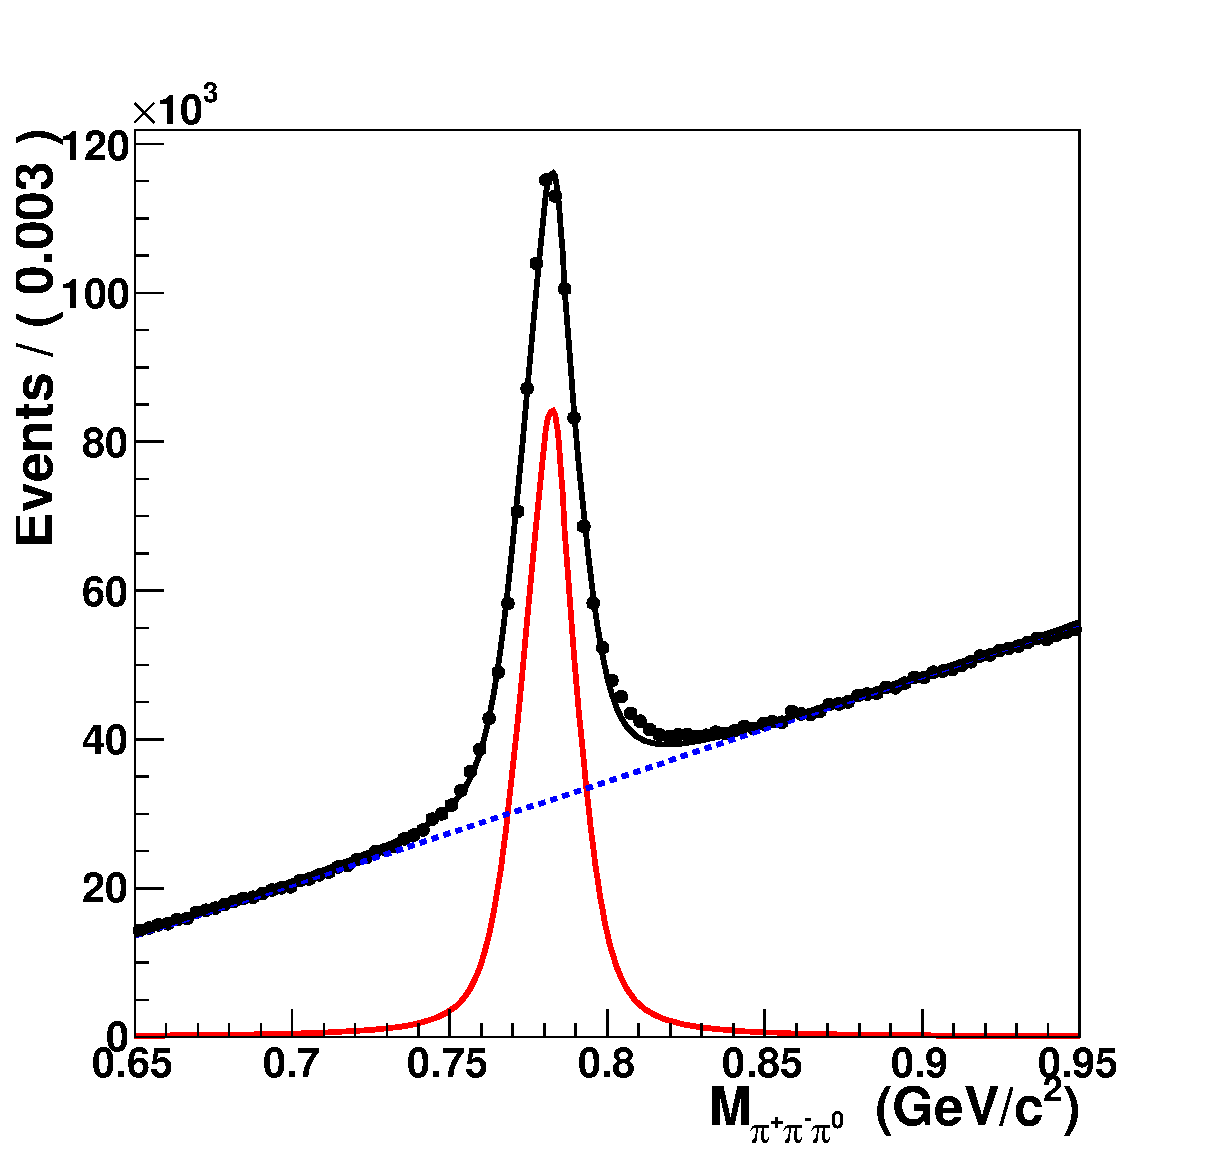
\includegraphics[width=0.5\textwidth]{graphics/data.eps}
		  \end{center}
\end{frame}
\begin{frame}{Data of $N^{obs}_{data}$, $N^{tot}_{data}$, $Br(\Omega\!\rightarrow\!3\pi)$ and $Br(\pi^0\!\rightarrow\!2\gamma)$}
From the fitting of data, we learn that\\
		 \begin{center}
		 $N^{obs}_{data}=7.01\times 10^5$.
			 \end{center}
		 And we learned from other's work that\\
		 \begin{center}
		 $N^{tot}_{data}=2.25 \times 10^8$.
			 \end{center}
		 \bigskip
As for $Br(\Omega\!\rightarrow\!3\pi)$ and $Br(\pi^0\!\rightarrow\!2\gamma)$, we can look them up in the PARTICLE PHYSICS BOOKLET.
\begin{center}
		 $Br(\Omega\!\rightarrow\!3\pi)=89.2\%$\\
		$Br(\pi^0\!\rightarrow\!2\gamma)=98.823\%$\\
		\end{center}
\end{frame}
\begin{frame}{Measure of the efficiency \epsilon}
 And the efficiency is calculated as\;  $\epsilon={N^{obs}_{sig}\over N^{tot}_{sig}},$\\
 which will be calculated via signal MC which was introduced before.\\
		\begin{columns}
		\begin{column}{0.4\textwidth}
		\begin{center}
 $N^{obs}_{sig}=1.8285\times 10^4$,
 \end{center}
 which is obtained from the fitting of signal MC, and\\
	  \begin{center}
	  $N^{tot}_{sig}=10^5$\\
	\end{center}
	as we set it to be.
\end{column}
   \begin{column}{0.5\textwidth}
 %  \begin{center}
   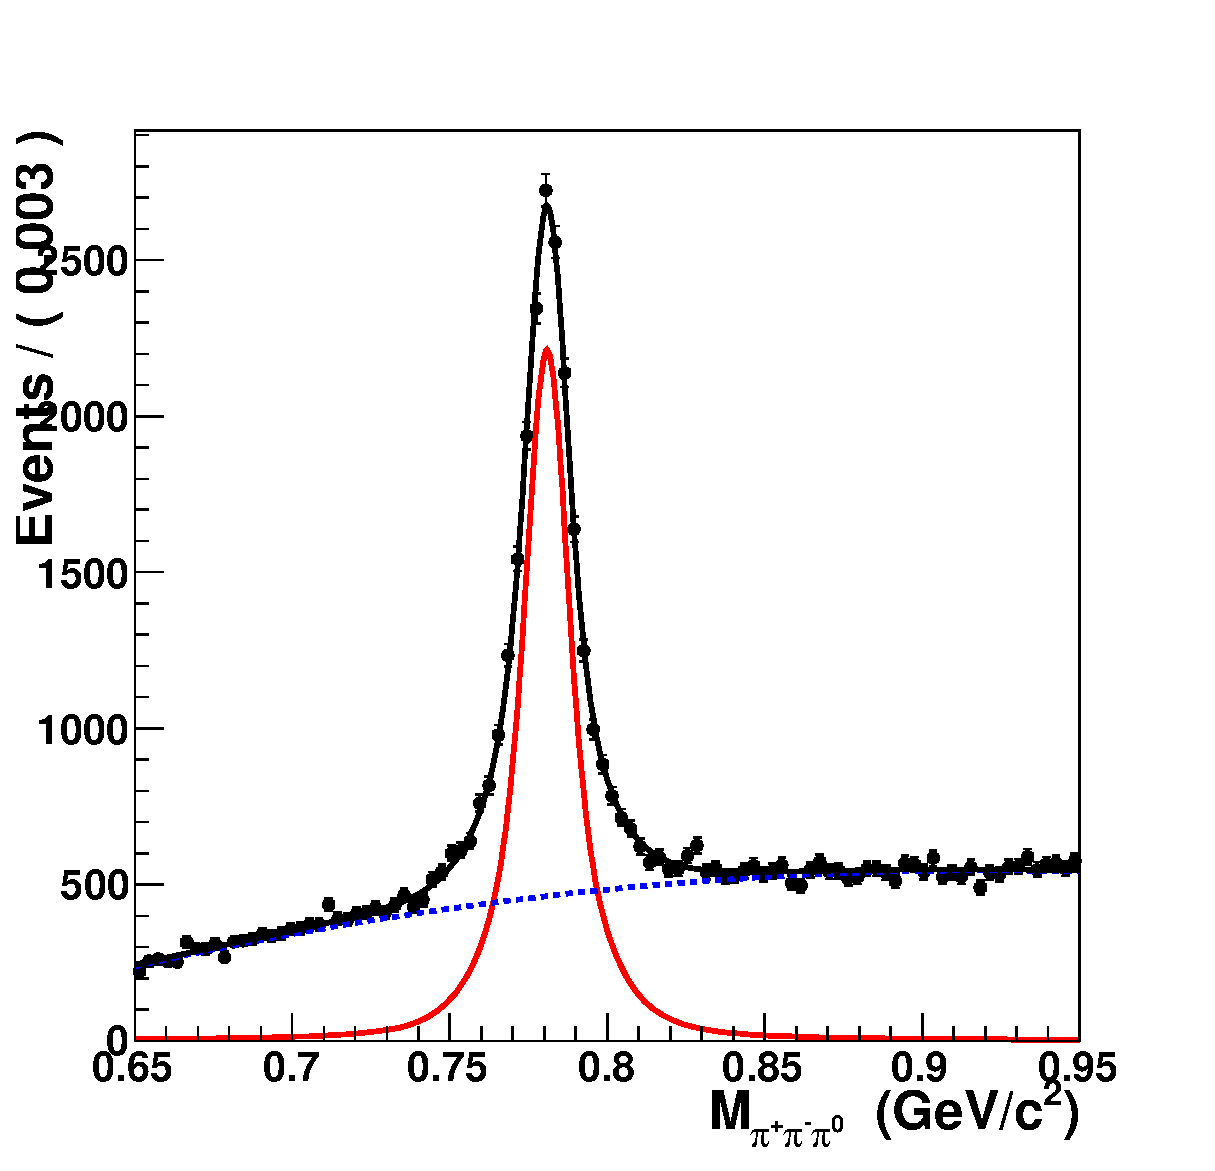
\includegraphics[width=0.8\textwidth]{graphics/signal.eps}
 %  \end{center}
 \end{column}
   \end{columns}
So we can get the efficiency as\\
	   \begin{center}
   $\epsilon=18.285\%$
   \end{center}
\end{frame}
\begin{frame}{Calculation of $Br(J\!/\!\psi\!\rightarrow\!\Omega\;4\pi)$}
With the formula ($*$), we can calculate $Br(J\!/\!\psi\!\rightarrow\!\Omega\;4\pi)$ as\\
\bigskip
\begin{center}
%\begin{equation}
$Br(J\!/\!\psi\!\rightarrow\!\Omega\;4\pi)={N^{obs}_{data} \over {N^{tot}_{data}\times Br(\Omega\!\rightarrow\!3\pi)\times Br(\pi^0\!\rightarrow\!2\gamma)\times \epsilon}}$\\
\bigskip
$~~~~~~~~~	=\frac{7.014\times10^5}{2.25\times 10^8 \times 89.2\% \times 98.823\% \times 18.285\%}$\\
\bigskip
$&=1.934\%$,\\
\end{center}
\bigskip
which almost equals to Ji Qingping's early work.
	\end{frame}
\section{Summary}
\begin{frame}{Summary}
\begin{itemize}
\item As you can see, I didn't not deal with errors analysis. Actually, every variable was measured or looked up with errors.\\
\bigskip
\item What was to be done is topology, which I didn't know very well.\\
\bigskip
\item What is to be done this term is mainly taking my course.\\
\end{itemize}
\end{frame}
\end{document}
